\section{Introduction}

In embedded and edge AI systems, a typical setup includes sensors that capture data from the physical world, software that processes this data, and actuators that execute actions based on computational outcomes. 
All processing tasks rely on specialized hardware optimized for efficiency and performance.

\begin{figure}[H]
    \centering
    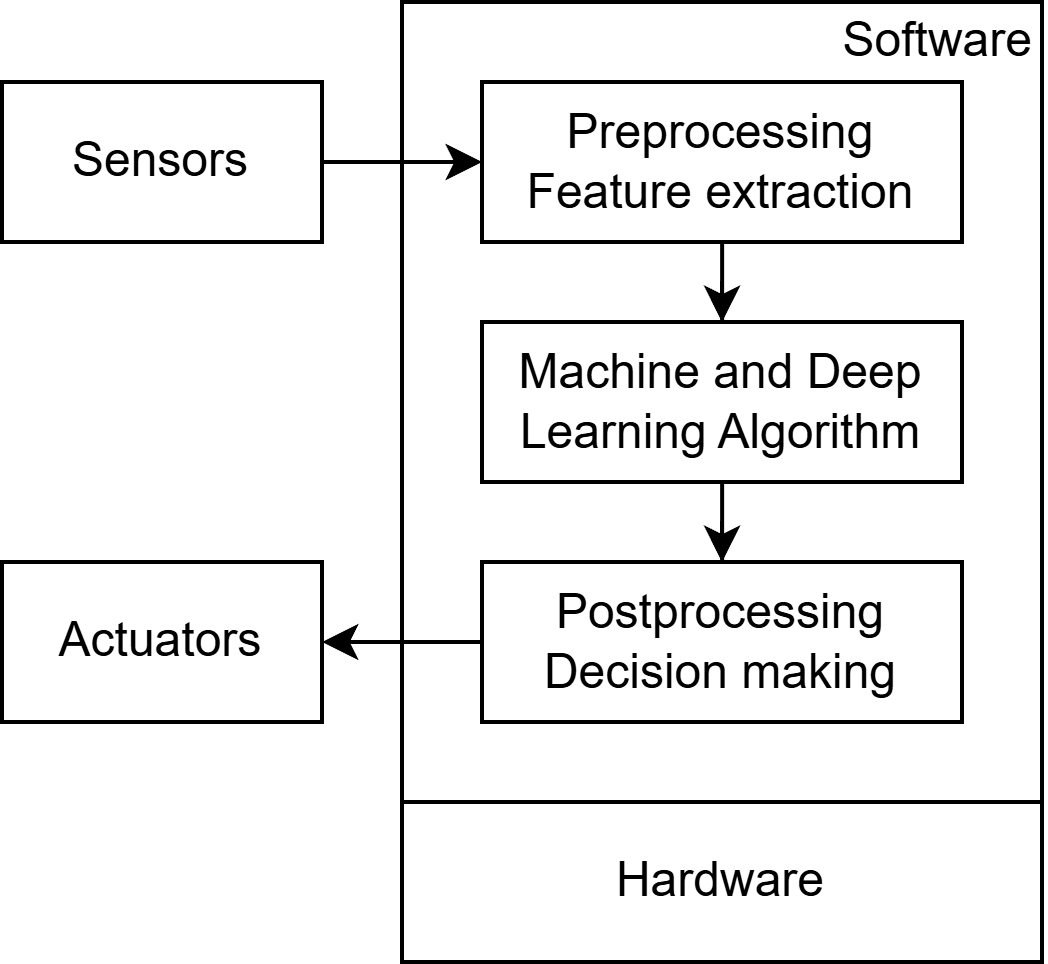
\includegraphics[width=0.5\linewidth]{images/eeai3.png}
    \caption{AI systems}
\end{figure}

Embedded systems are computers designed to control and manage the electronics within various physical devices. 
Embedded software refers to the programs that run on these systems, enabling their functionality.

Unlike general-purpose computers such as laptops or smartphones, embedded systems are typically designed for a specific, dedicated task, ensuring optimized performance, reliability, and energy efficiency for their intended application.